% Die folgenden zwei Befehle binden die CoderDojo-Styles ein.
		
\newcommand*{\VorlagenPfad}{../Vorlagen}	
\documentclass{\VorlagenPfad/coderdojokatext}

% Titel als Kommando für den Header/Footer definieren
\renewcommand{\Titel}{Raspberry Pi - Workshop I}
\usepackage{hyperref}

\usepackage[figurename=Abb.]{caption}

\begin{document}

% Titel anzeigen und um den Header/Footer zu generieren
\begin{center}
	{\huge \Titel}
\end{center}

\begin{minipage}[t]{0.45\linewidth}
Hallo TExt
\end{minipage}

\begin{figure}[htb]
	\centering
	\begin{minipage}[t]{0.45\linewidth}
		\centering
		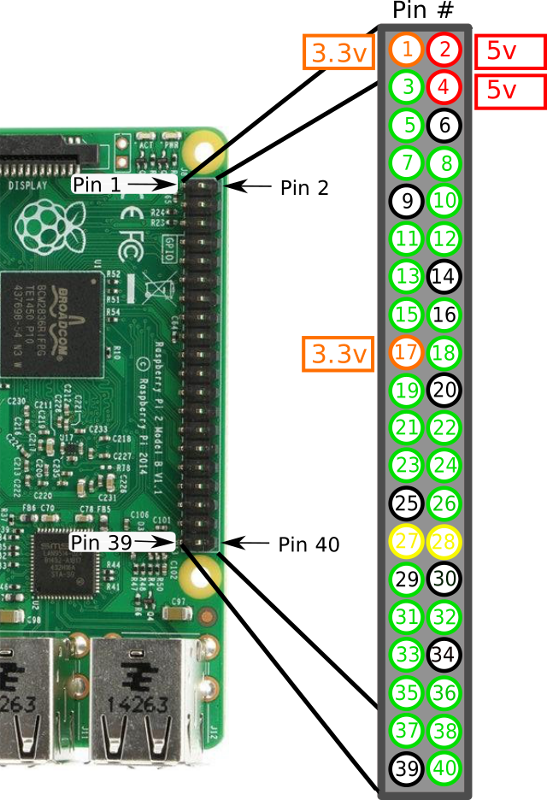
\includegraphics[width=.9\textwidth]{pin_layout.png}
		\caption{Raspberry Pi Pin-Übersicht}
	\end{minipage}% <- sonst wird hier ein Leerzeichen eingefügt
	\hfill
	\begin{minipage}[t]{0.45\linewidth}
		\centering
		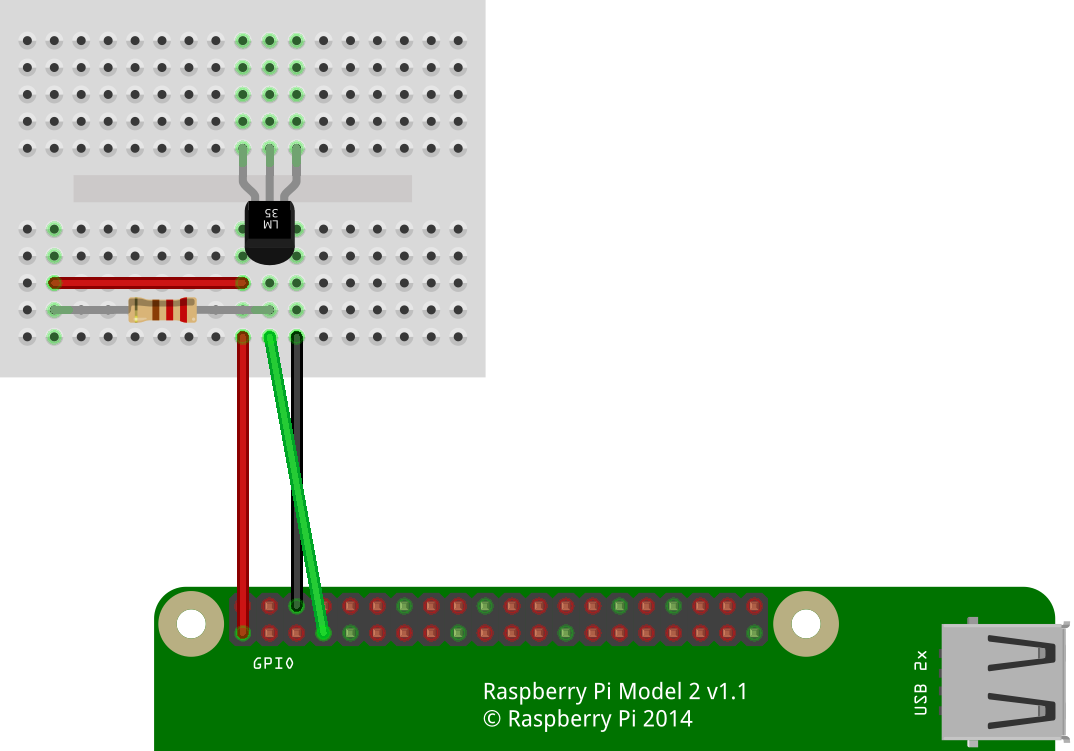
\includegraphics[width=.9\textwidth]{temperatur/temperatur.png}
		\caption{Temperaturmessung}
	\end{minipage}
\end{figure}



\begin{figure}[htb]
	\centering
	\begin{minipage}[t]{0.45\linewidth}
		\centering
		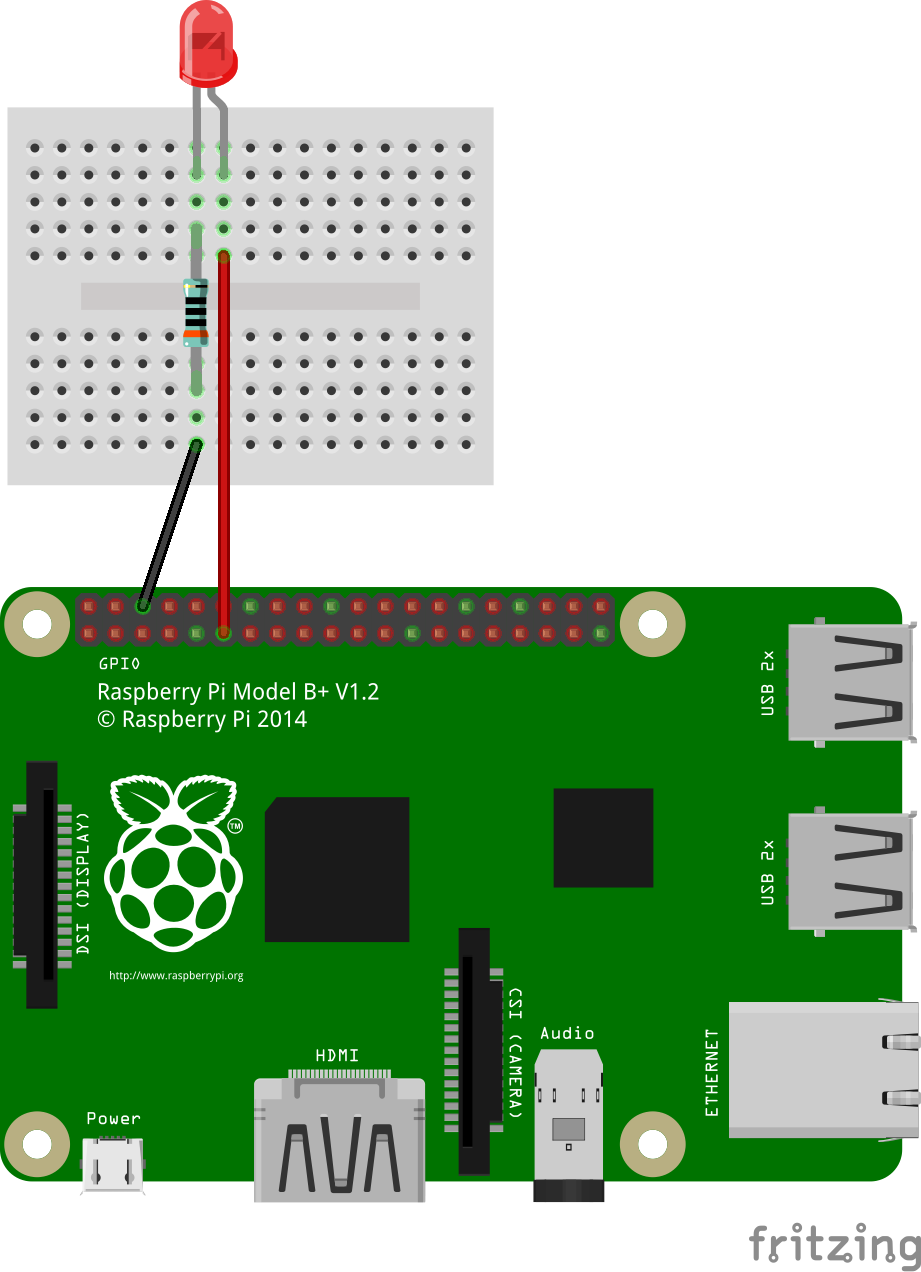
\includegraphics[width=.9\textwidth]{ampel/eine_led_bb.png}
		\caption{Schaltung mit einer LED}
	\end{minipage}% <- sonst wird hier ein Leerzeichen eingefügt
	\hfill
	\begin{minipage}[t]{0.45\linewidth}
		\centering
		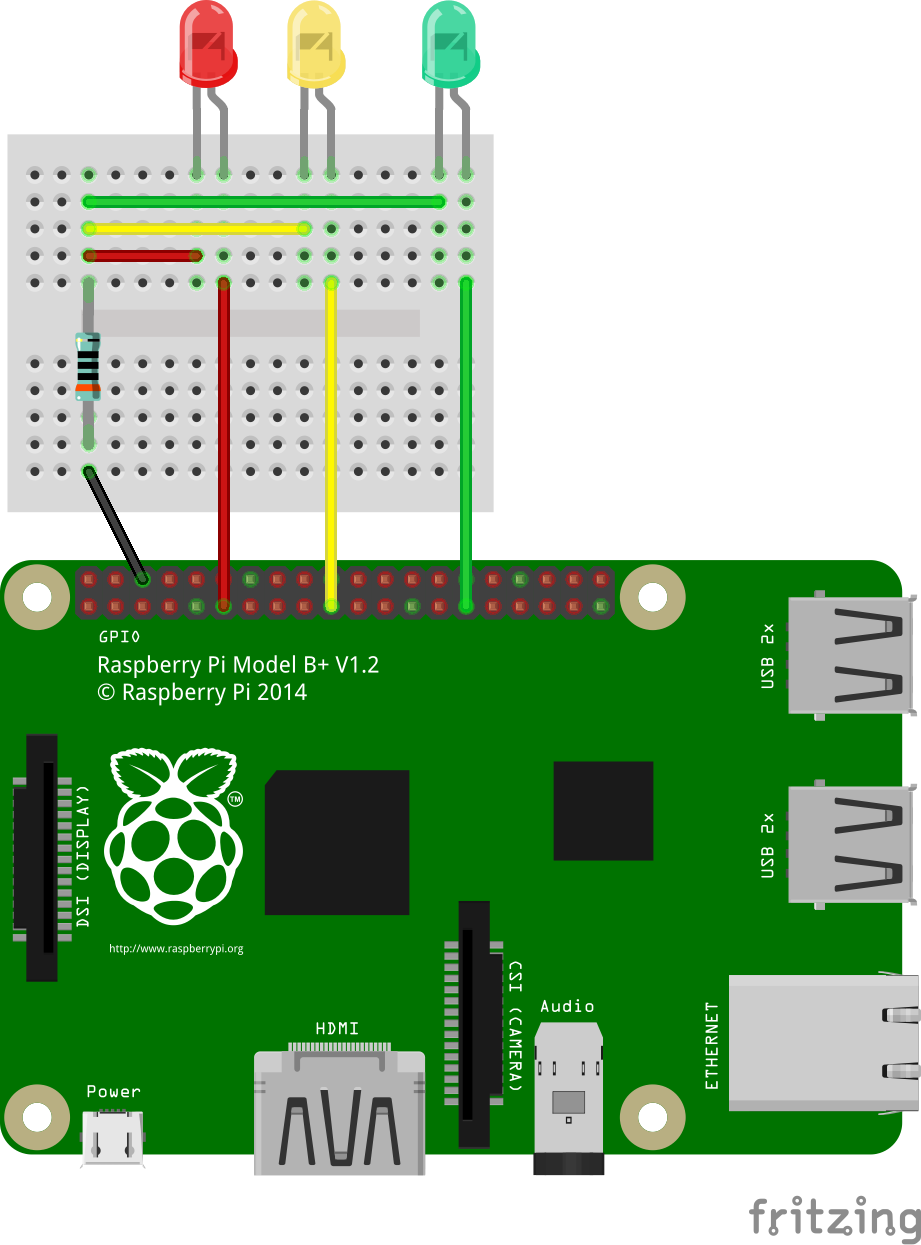
\includegraphics[width=.9\textwidth]{ampel/ampel_bb.png}
		\caption{Ampelschaltung mit 3 LEDs}
	\end{minipage}
\end{figure}





\end{document}